\section{Methods}\label{meth}
\paragraph{Data Source}
Full details of the FSW survey methodology are available in \cite{Yam2013}.
Briefly, 328 women aged 15+
who reported exchanging or selling sex for money, favors, or goods in the past 12 months
were recruited via respondent-driven sampling (RDS) \cite{Heckathorn1997}.   
\begin{figure}
  \begin{subfigure}[b]{\textwidth}
    \centering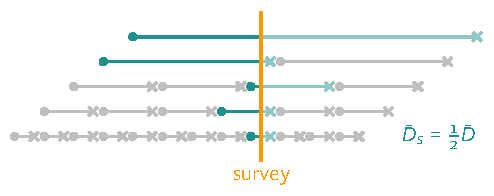
\includegraphics[scale=1]{diag.yss.censor}
    \caption{Right censoring of reported durations selling sex in a steady state population}
    \label{fig:diag.yss.censor}
  \end{subfigure}
  \begin{subfigure}[b]{\textwidth}
    \centering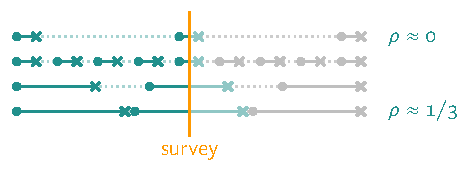
\includegraphics[scale=1]{diag.yss.gaps}
    \caption{Possible periods of selling sex for one individual who stopped selling sex at least once}
    \label{fig:diag.yss.gaps}
  \end{subfigure}
  \begin{subfigure}[b]{\textwidth}
    \centering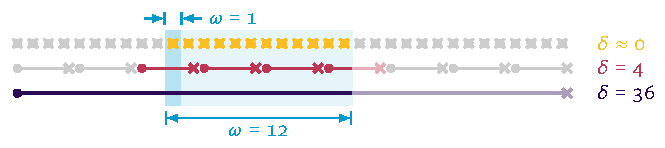
\includegraphics[scale=1]{diag.partner.types}
    \caption{Differences in partnership duration \vs recall period}
    \label{fig:diag.partner.types}
  \end{subfigure}
  \begin{subfigure}[b]{\textwidth}
    \centering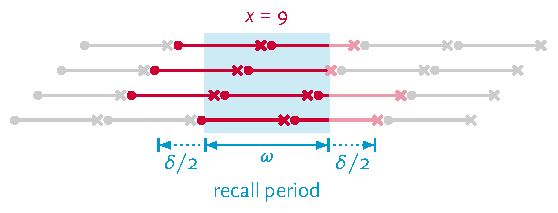
\includegraphics[scale=1]{diag.partners}
    \caption{Fully and partially observed partnerships during a given recall period}
    \label{fig:diag.partners}
  \end{subfigure}
  \caption{Diagrams of fully observed, censored, and unobserved periods
    selling sex or within ongoing sexual partnerships}
  \label{fig:diag}
    \floatfoot{Guide:
    \g{$\bullet$\,}{start}, \g{$\bm{\times}$\,}{end},
    \g{green}{selling sex}, \g{red}{ongoing partnership},
    \g{yellow}{survey / recall period},
    \g{colour}{fully observed}, \g{faded colour}{right censored}, \g{grey}{unobserved},
    \g{$\bar{D}_s$} and \g{overall}{$\bar{D}$}{mean duration at survey},
    \g{$\rho$}{proportion of total period in most recent period},
    \g{$\omega$}{recall period}, \g{$\delta$}{partnership duration},
    \g{$x$}{number of reported partnerships}.}
\end{figure}
%===================================================================================================
\subsection{Risk Group Duration}\label{meth.yss} %SM: i really like the structure/subheading organizations - made it nice and easy to follow
The FSW survey \cite{Baral2014} included questions about
the current respondent's age and the age of first selling sex.
The difference between these ages could be used to define a crude ``duration selling sex''.
Using this approach, the median unadjusted duration among FSW in Eswatini was 4 years.
However, this estimate can be improved by considering the following potential biases.
\paragraph{Distribution}
In compartmental transmission models, %SM: mention compartmental models in introduction. woudl the bias-adjustments only refer to compartmental models or also ABM? lets make it easier for reader so they don't ask this question while reading the methods part :) 
durations are implicitly assumed to be exponentially distributed \cite{?}.
This assumption was found to be reasonable here (see Figure~\ref{fig:yss.fit}),
but the median of an exponential distribution is less than the mean
by a factor of $\distr{log}{2}$ due to skewness.
Thus, the unadjusted mean duration could be estimated from the median as
$\bar{D}_{s} = 4/\distr{log}{2} = 5.77$.
\paragraph{Sampling}
Sampling error was considered via RDS-adjustment in \cite{Baral2014},  %SM: agree with using RDS acronym b/c we have to keep saying RDS-adjusted (and also RDS is commonly used in general, topic-agnostic epi language),  but try to avoid using acronyms if possible - I think we should not not use FSW, for example. 
yielding estimates of the proportions of FSW
who had sold sex starting 0--2, 3--5, 6--10, and 11+ years ago.
The adjusted proportions indicate fewer years selling sex \vs the unadjusted proportions,
which would be consistent with
challenges in reaching women in the first year(s) of sex work \cite{Cheuk2020}.
Fitting an exponential distribution to the cumulative adjusted proportions
(methods in Appendix~\ref{app.yss}; result in Figure~\ref{fig:yss.fit})
yielded an estimated distribution mean $\bar{D}_s$ of 4.1 (\ci: 3.4,~4.9) years.
% TODO: describe fitting methods (app)
\paragraph{Censoring}
These crude durations are considered right censored %SM: for consitency and easier for reader, lets try to stick to same words (crude, etc.) throughout unless we meant something different by "reported"?
because they only capture engagement in sex work up until data collection, and 
thus do not include sex work that occurs after the time of data collection  %SM: rephrase to be less of a "definitive-sounding". 
(Figure~\ref{fig:diag.yss.censor}) \cite{Fazito2012}.
If we assume that the survey reaches FSW
at a random time point during their total (eventual) duration selling sex $D$,
then the duration reported in the survey can be effectively considered $D_s \sim \distr{Unif}{0,D}$.
Thus, the mean duration reported in the survey is $\bar{D}_s = \frac12 \bar{D}$,
and we can define $f = \bar{D} / \bar{D}_s = 2$,
to give a further adjusted estimate as: $\bar{D} = f\bar{D}_s$.
In case the RDS-adjustment did not fully account for delayed self-identification as FSW,
we could use $f \sim \distr{Unif}{1.5,2}$, or similar.
\paragraph{Measurement}
Finally, FSW may not sell sex continuously.
The 2011 survey did not ask whether respondents ever stopped selling sex. 
Other data from a 2014 survey of FSW in Eswatini suggest that $\phi = 45\%$ had stopped at least once \cite{EswKP2014}.  %SM: since  didn't talk about the 2014 survey in the methods/intro, so rephrase to say - other surveys/data indicate that... I would bring this up later in the paragraph - as its hard to follow which survey we are talking about in the next sentence?
% TODO: not reported in EswKP2014
Among the respondents who stopped, we have no further information about
the proportion of the total period (\ie since first started selling sex)
reflected in the current period (\ie since re-starting most recently). %SM: from which source? the 2011 or 2014 survey? 
We denote this proportion $\rho$, and define the expected value for two extreme cases
(Figure~\ref{fig:diag.yss.gaps} top and bottom):
respondents were almost \emph{never} selling sex during the total period ($\rho = 0$), or
respondents were almost \emph{always} selling sex ($\rho = 1/3$).
As shown in Figure~\ref{fig:diag.yss.gaps},
the expected value for $\rho$ given multiple stoppages is contained within these extremes.
A strongly uninformative prior could then be $\rho \sim \distr{Unif}{0,1/3}$.
Thus, we can define the final adjusted estimate for duration in sex work as:
$\bar{D} = f[(1-\phi)+(\phi)\rho]\bar{D}_s$, with
$\phi = 0.45$, $\rho \sim \distr{Unif}{0,1/3}$, and $f \sim \distr{Unif}{1.5,2}$.
%===================================================================================================
\subsection{Rates of Partnership Change}\label{meth.partners}
The FSW survey \cite{Baral2014} also asked respondents to report  %SM: the 2011 survey yes?
their numbers of sexual partners in the past 30 days,
stratified by three types of partner:
new paying clients, regular paying clients, and non-paying partners.
Our aim is to use the mean numbers of reported partners ($x$) %SM: avoid term "aim" so that "aim" only applies to what we said in introduction
for the 30-day recall period ($\omega$),
with the assumed partnership durations below ($\delta$),
to define expected rates of partnership change ($Q$).
We also explore the expected number of current partners ($K$) below. %SM: below refers to which section?
We focus on means (not distributions), since
rates of partnership change for each population are assumed to be
homogeneous in compartmental transmission models. %SM, after reading through - yes, we should mention comparatmental models in intro :) 
Given the assumptions below, we adjust for sampling and measurement bias
to arrive at the final estimates.
\paragraph{Assumptions} %SM: very nice section
We assume that
only a small proportion of new clients go on to become regular clients;
thus, we conceptualize ``new'' clients as effectively ``one-off'' clients.
Since no survey questions asked about partnership durations,
we further assume that partnership durations were:
1~day with new paying clients,
4~months with regular paying clients, and
3~years with non-paying partners.
% TODO: cite?
\paragraph{Sampling}  %SM: fantastic figures! very clear
RDS-adjusted proportions of respondents reporting different numbers of partners
were drawn from \cite{Baral2014}.
Following a similar approach as before (details in Appendix~\ref{app.partners}),
the mean numbers of reported partners of each type
were estimated from these proportions as mean (\ci):
2.52~(2.31,~2.75) new clients,
5.83~(5.15,~6.48) regular clients, and
1.38~(1.23,~1.52) non-paying partners
(Figure~\ref{fig:partners.fit}).
\paragraph[?]{Rate or Number}
Numbers of reported partners have generally been interpreted in two ways ---
$x/\omega$ as the \emph{rate} of partnership change ($Q$) or
$x$ as the \emph{number} of current partners ($K$):
\begin{subequations}\label{eq:bQK}
\begin{alignat}{1}
  Q &\approx \frac{x}{\omega}\\
    &\text{or} \nonumber\\
  K &\approx x
\end{alignat}
\end{subequations}
Both interpretations are reasonable under certain conditions:
If partnership duration is short and the recall period is long ($\delta \ll \omega$),
then reported partnerships mostly reflect \emph{complete} partnerships,
and thus $x/\omega \approx Q$.
If partnership duration is long and the recall period is short ($\delta \gg \omega$),  %SM: could we give an example to make it tangilble (e.g. 10 years, and 6 months in the context of FSW surveys,....)
then reported partnerships mostly reflect \emph{ongoing} partnerships,
and thus $x \approx K$.
However, if partnership duration and recall period are similar in length ($\delta \approx \omega$),
then reported partnerships reflect a mixture of tail-ends, complete, and ongoing partnerships,
and thus $x/\omega$ overestimates $Q$, but $x$ also overestimates $K$.
These three cases are illustrated in Figure~\ref{fig:diag.partner.types}.
Note that all estimates using \eqref{eq:bQK} are biased via this same mechanism,
just that some biases are larger than others.
\paragraph{Adjustment}
The bias-adjustment starts by first assuming that survey timing is
effectively random with respect to the durations of interest.
Then, if either end of the recall period would capture an ongoing partnership,
the intersection point would be, on average, at the partnership mid-point. %SM: rephrase for a bit more clarity / simplicty - may need to break down into 2 sentences...
Thus, the recall period is extended
by half the partnership duration $\delta/2$ on each end, and $\delta$ overall,
as illustrated in Figure~\ref{fig:diag.partners}.
We can then define unbiased estimators of $Q$ and $K$ as:
\begin{subequations}\label{eq:uQK}
\begin{alignat}{1}
  Q &= \frac{x}{\omega + \delta}\\
  K &= \frac{x \delta}{\omega + \delta} = Q \delta
\end{alignat}
\end{subequations}
To further reflect uncertainty in these estimates [TODO]. %SM: have not reviewed this section yet
% NOTE: current simulation is a bit circular and needs revision
%       it does not actually calculate p(Q|x) but instead uses p(x|Q)
%       see: https://stats.stackexchange.com/questions/620805
We then compared biased \vs unbiased estimates of $Q$ and $K$
via \eqref{eq:bQK} \vs \eqref{eq:uQK}, for each partnership type.
\paragraph{Generalized Trends}
To illustrate more general trends in the magnitude of bias,
we further compared biased \vs unbiased estimates of $Q$ and $K$ across
a range of different partnership durations $\delta \in [0.1, 10]$ and
recall periods $\omega \in [0.1, 10]$,
with fixed true rate $Q = 1$ (arbitrary units).
